%%%%%%%%%%%%%%%%%%%%%%%%%%%%%%%%%%%%%%%%%
% Beamer Presentation
% LaTeX Template
% Version 1.0 (10/11/12)
%
% This template has been downloaded from:
% http://www.LaTeXTemplates.com
%
% License:
% CC BY-NC-SA 3.0 (http://creativecommons.org/licenses/by-nc-sa/3.0/)
%
%%%%%%%%%%%%%%%%%%%%%%%%%%%%%%%%%%%%%%%%%

%----------------------------------------------------------------------------------------
%	PACKAGES AND THEMES
%----------------------------------------------------------------------------------------

\documentclass{beamer}

\mode<presentation> {

% The Beamer class comes with a number of default slide themes
% which change the colors and layouts of slides. Below this is a list
% of all the themes, uncomment each in turn to see what they look like.

%\usetheme{default}
%\usetheme{AnnArbor}
%\usetheme{Antibes}
%\usetheme{Bergen}
%\usetheme{Berkeley} % Neat Contents on left
%\usetheme{Berlin}
%\usetheme{Boadilla}
%\usetheme{CambridgeUS} % Neat but breadcrumbs at top
%\usetheme{Copenhagen}
%\usetheme{Darmstadt}
%\usetheme{Dresden}
%\usetheme{Frankfurt}
%\usetheme{Goettingen} %Neat contents on right
\usetheme{Hannover} %Neat contents on left
%\usetheme{Ilmenau}
%\usetheme{JuanLesPins}
%\usetheme{Luebeck}
%\usetheme{Madrid}
%\usetheme{Malmoe}
%\usetheme{Marburg} % Contents on right in contrast color
%\usetheme{Montpellier}
%\usetheme{PaloAlto} % Contents on left
%\usetheme{Pittsburgh}
%\usetheme{Rochester}
%\usetheme{Singapore}
%\usetheme{Szeged}
%\usetheme{Warsaw}

% As well as themes, the Beamer class has a number of color themes
% for any slide theme. Uncomment each of these in turn to see how it
% changes the colors of your current slide theme.

%\usecolortheme{albatross}
%\usecolortheme{beaver}
%\usecolortheme{beetle}
%\usecolortheme{crane}
%\usecolortheme{dolphin}
%\usecolortheme{dove}
%\usecolortheme{fly}
%\usecolortheme{lily}
%\usecolortheme{orchid}
%\usecolortheme{rose}
%\usecolortheme{seagull}
\usecolortheme{seahorse}
%\usecolortheme{whale}
%\usecolortheme{wolverine}

%\setbeamertemplate{footline} % To remove the footer line in all slides uncomment this line
%\setbeamertemplate{footline}[page number] % To replace the footer line in all slides with a simple slide count uncomment this line

%\setbeamertemplate{navigation symbols}{} % To remove the navigation symbols from the bottom of all slides uncomment this line
}

\usepackage{graphicx} % Allows including images
\usepackage{booktabs} % Allows the use of \toprule, \midrule and \bottomrule in tables

%----------------------------------------------------------------------------------------
%	TITLE PAGE
%----------------------------------------------------------------------------------------

\title[Improving Outcomes in Pancreatic Surgery]{An investigation of the clinical utility of preoperative cardiopulmonary exercise testing in patients undergoing major pancreatic surgery.} % The short title appears at the bottom of every slide, the full title is only on the title page

\author{Vishnu V Chandrabalan} % Your name
\institute[UoG] % Your institution as it will appear on the bottom of every slide, may be shorthand to save space
{
University of Glasgow \\ % Your institution for the title page
\medskip
% \textit{john@smith.com} % Your email address
}
\date{\today} % Date, can be changed to a custom date

\begin{document}

\begin{frame}
\titlepage % Print the title page as the first slide
\end{frame}

\begin{frame}
\frametitle{Overview} % Table of contents slide, comment this block out to remove it
\tableofcontents % Throughout your presentation, if you choose to use \section{} and \subsection{} commands, these will automatically be printed on this slide as an overview of your presentation
\end{frame}

%----------------------------------------------------------------------------------------
%	PRESENTATION SLIDES
%----------------------------------------------------------------------------------------

%------------------------------------------------
\section{Introduction}
\subsection{Pancreatic cancer}
\begin{frame}
	\frametitle{Pancreatic cancer} %Epidemiology/outcomes
	\begin{block}{The Problem}
		\begin{itemize}
			\item 10th common cancer but 5th common cause of cancer death
			\item Survival	1-yr: 20.8\%, 5-yr: 3.3\%, 10yr: 1.1\%
			\item Operable disease : approx 15\%
		\end{itemize}
	\end{block}
	\begin{block}{Treatment}
		\begin{itemize}
			\item Surgery is the primary modality of cure
			\item Adjuvant chemotherapy has an important role in improving survival
		\end{itemize}
	\end{block}
	\begin{block}{Pancreaticoduodenectomy}
		\begin{itemize}
			\item Complex surgery with 50\% morbidity
			\item Performed only in specialist centres
			\item Patient fitness is as important as tumour factors
		\end{itemize}
	\end{block}
\end{frame}

\begin{frame}
	\frametitle{Preoperative Risk Stratification} 
	
\end{frame}

\subsection{CPET}

\begin{frame}
	\frametitle{Basis of CPET - Cellular Respiration} 
	\begin{figure}
		\centering
		\includegraphics[width=0.7\linewidth]{CellRespiration}
		\caption[Cellular Respiration]{Cellular Respiration}
		\label{fig:CellRespiration}
	\end{figure}
\end{frame}

\begin{frame}
	\frametitle{CPET and Body Composition}
\end{frame}

\subsection{Jaundice}

\begin{frame}
	\frametitle{The Jaundiced Patient}
\end{frame}

\subsection{Inflammation}


\section{Results}
\subsection{CPET vs Outcomes}
\begin{frame}
	\frametitle{CPET and Postoperative Outcomes}
\end{frame}

\subsection{CPET vs Jaundice}
\begin{frame}
	\frametitle{CPET and Jaundice}
\end{frame}

\subsection{CPET vs Body Composition}
\begin{frame}
	\frametitle{CPET and Body Composition}
\end{frame}

\subsection{Systemic inflammation}

\begin{frame}
	\frametitle{Preop Pathophysiology and Postoperative Systemic Inflammation}
	\begin{block}{title}
		Preoperative inflammatory status of the patient and obstructive jaundice play an important role in modulating postoperative systemic inflammation which may not simply be due to the effect of surgery and its sequelae.
	\end{block}
\end{frame}

\begin{frame}
	\frametitle{Postoperative Systemic Inflammation and Outcomes}
\end{frame}




\begin{frame}
\frametitle{Multiple Columns}
\begin{columns}[c] % The "c" option specifies centered vertical alignment while the "t" option is used for top vertical alignment

\column{.45\textwidth} % Left column and width
\textbf{Heading}
\begin{enumerate}
\item Statement
\item Explanation
\item Example
\end{enumerate}

\column{.5\textwidth} % Right column and width
Lorem ipsum dolor sit amet, consectetur adipiscing elit. Integer lectus nisl, ultricies in feugiat rutrum, porttitor sit amet augue. Aliquam ut tortor mauris. Sed volutpat ante purus, quis accumsan dolor.

\end{columns}
\end{frame}

\begin{frame}
\frametitle{Table}
\begin{table}
\begin{tabular}{l l l}
\toprule
\textbf{Treatments} & \textbf{Response 1} & \textbf{Response 2}\\
\midrule
Treatment 1 & 0.0003262 & 0.562 \\
Treatment 2 & 0.0015681 & 0.910 \\
Treatment 3 & 0.0009271 & 0.296 \\
\bottomrule
\end{tabular}
\caption{Table caption}
\end{table}
\end{frame}

%------------------------------------------------

\begin{frame}
\frametitle{Oxygen Delivery}
\begin{theorem}[Mass--energy equivalence]
$E = mc^2$
\end{theorem}
\end{frame}

%------------------------------------------------

\begin{frame}[fragile] % Need to use the fragile option when verbatim is used in the slide
\frametitle{Verbatim}
\begin{example}[Theorem Slide Code]
\begin{verbatim}
\begin{frame}
\frametitle{Theorem}
\begin{theorem}[Mass--energy equivalence]
$E = mc^2$
\end{theorem}
\end{frame}\end{verbatim}
\end{example}
\end{frame}

%------------------------------------------------

\begin{frame}
\frametitle{Figure}
Uncomment the code on this slide to include your own image from the same directory as the template .TeX file.
%\begin{figure}
%\includegraphics[width=0.8\linewidth]{test}
%\end{figure}
\end{frame}

%------------------------------------------------

\begin{frame}[fragile] % Need to use the fragile option when verbatim is used in the slide
\frametitle{Citation}
An example of the \verb|\cite| command to cite within the presentation:\\~

This statement requires citation \cite{p1}.
\end{frame}

%------------------------------------------------

\begin{frame}
\frametitle{References}
\footnotesize{
\begin{thebibliography}{99} % Beamer does not support BibTeX so references must be inserted manually as below
\bibitem[Smith, 2012]{p1} John Smith (2012)
\newblock Title of the publication
\newblock \emph{Journal Name} 12(3), 45 -- 678.
\end{thebibliography}
}
\end{frame}

%------------------------------------------------

\begin{frame}
\Huge{\centerline{The End}}
\end{frame}

%----------------------------------------------------------------------------------------

\end{document} 